\chapter{Specifikacija programske potpore}
		
		\section{Funkcionalni zahtjevi}
		
		
		\noindent \textbf{Dionici:}
		
		\begin{packed_enum}
			
			\item Klijent teretane
			\begin{packed_enum}
				
				\item registrirani
				\item neregistrirani
				
			\end{packed_enum}
			\item Trener
			\item Voditelj teretane			
			\item Administrator
			\item Razvojni tim
			
		\end{packed_enum}
		
		\noindent \textbf{Aktori i njihovi funkcionalni zahtjevi:}
		
		
		\begin{packed_enum}
			\item  \underbar{Neregistrirani/neprijavljeni korisnik (inicijator) može:}
			
			\begin{packed_enum}
				
				\item pregledati popis svih teretana na platformi
				\item sortirati spomenuti popis prema sljedećim kriterijima: ime teretane, lokacija, trener
				\item otvoriti početnu stranicu svake teretane na kojoj se nalaze osnovne informacije (radno vrijeme, lokacija, cijena
				članarine…)
				\item izraditi administratorski, voditeljski, trenerski ili korisnički račun s namjerom treniranja u teretani za koje je potrebno navesti ime, prezime i email adresu, dok se može, ali ne mora dodati PayPal račun te je za izradu trenerskog korisničkog računa posebno potrebno navesti posebne podatke poput visine i težine
				
				
			\end{packed_enum}
			
			\item  \underbar{Klijent (inicijator) može:}
			
			\begin{packed_enum}
				
				\item pregledavati i sortirati popis registriranih teretana
				\item pregledavati i mijenjati osobne podatke
				\item izbrisati svoj korisnički račun
				\item plaćati članarine u teretanama putem interneta
				\item pregledavati sve izvršene transakcije u kojima su sudjelovali
				\item pregledavati popis teretana u kojima smiju vježbati, odnosno u kojima su platili članarinu
				\item kupovati planove prehrane i vježbanja od trenera
				\item ugovarati privatne ili grupne treninge
				\item voditi i pratiti napredak u vlastitom planu vježbanja
				
			\end{packed_enum}
			
			\item  \underbar{Trener (inicijator) može:}
			
			\begin{packed_enum}
				
				\item pregledavati i sortirati popis registriranih teretana
				\item pregledavati i mijenjati osobne podatke
				\item izbrisati svoj korisnički račun
				\item objavljivati ponude planova treninga i/ili vježbanja
				\item objavljivati i ugovarati termine privatnih i grupnih treninga u teretanama gdje imaju te ovlasti
				\item pregledavati sve izvršene transakcije u kojima su sudjelovali
				\item pregledavati popis teretana u kojima smiju djelovati, odnosno raditi (voditi treninge, planovi prehrane i sl.)
				\item nuditi usluge treniranja teretanama
				
			\end{packed_enum}
			
			\item  \underbar{Voditelj teretane (inicijator) može:}
			
			\begin{packed_enum}
				
				\item pregledavati i sortirati popis registriranih teretana
				\item pregledavati i mijenjati osobne podatke
				\item izbrisati svoj korisnički račun
				\item stvarati nove teretane u sustavu
				\item davati dozvolu drugim voditeljima da vode neke njegove teretane
				\item mijenjati važne informacije o teretanama (radno vrijeme, lokacija i sl.)
				\item dopuštati registriranim trenerima rad u teretanama koje vodi
				\item vidjeti sve izvršene transakcije na aplikaciji unutar vlastite teretane
				
			\end{packed_enum}
			
			\item  \underbar{Administrator (inicijator) može:}
			
			\begin{packed_enum}
				
				\item pregledavati i sortirati popis registriranih teretana
				\item pregledavati i mijenjati osobne podatke
				\item vidjeti sve korisničke račune
				\item izbrisati svoj korisnički račun
				\item stvarati nove i brisati postojeće teretane u sustavu
				\item pregledati sve izvršene transakcije u aplikaciji
				\item davati dozvolu  voditeljima da vode pojedine teretane
				\item mijenjati važne informacije o teretanama (radno vrijeme, lokacija i sl.)
				\item dopuštati registriranim trenerima rad u teretanama
				
			\end{packed_enum}
			
			
			\item  \underbar{Baza podataka (sudionik):}
			
			\begin{packed_enum}
				
				\item pohranjuje sve podatke o korisnicima
				\item čuva informacije o ulogama pojedinih korisnika
				\item pohranjuje podatke o svim teretanama, njihovim voditeljima, trenerima i članovima
				\item pohranjuje izvršene transakcije
				
			\end{packed_enum}
			
		\end{packed_enum}
		
		\eject
				
			\subsection{Obrasci uporabe}
				
				\textbf{\textit{dio 1. revizije}}
				
				\subsubsection{Opis obrazaca uporabe}


					\noindent \underbar{\textbf{UC1 - Pregled teretana}}
					\begin{packed_item}
	
						\item \textbf{Glavni sudionik: }neregistrirani korisnik, klijent, trener, voditelj teretane i administrator
						\item  \textbf{Cilj:} Pregled teretana
						\item  \textbf{Preduvjet:} -

						\item  \textbf{Opis osnovnog tijeka:}
						
						\item[] \begin{packed_enum}
	
							\item Prikazan popis teretana
							\item Korisnik može tražit teretane (prema nekim kriterijima - search)
							\item Korisnik može birati teretanu o kojoj će dobiti informacije
						\end{packed_enum}
						\end{packed_item}
						
						
						\noindent \underbar{\textbf{UC2 - Registracija korisnika}}
					\begin{packed_item}
	
						\item \textbf{Glavni sudionik: }Neregistrirani korisnik
						\item  \textbf{Cilj:} Izrada korisničkog računa kojim korisnik dobiva dodatne funkcionalnosti sustava
						\item  \textbf{Sudionici:} Baza podataka
						\item  \textbf{Preduvjet:} -
						\item  \textbf{Opis osnovnog tijeka:}
						
						\item[] \begin{packed_enum}
	
							\item Neprijavljeni korisnik odabire opciju registracije
							\item Neprijavljeni korisnik unosi potrebne podatke
							\item Korisnik prima obavijest o uspješnoj registraciji
						\end{packed_enum}
					
						\item  \textbf{Opis mogućih odstupanja:}
						
						\item[] \begin{packed_item}
	
							\item[-]
							Odabir zauzetog korisničkog imena ili e-maila, odabir nepostojećeg e-maila ili nedozvoljen format unosa nekog od podataka
							\item[] \begin{packed_enum}
								
								\item Sustav neprijavljenom korisniku šalje objavu o neuspješnoj registraciji te ga vraća na početnu stranicu za registraciju
								\item Korisnik mijenja neispravne podatke i završava unos ili odustaje od registriranja
								
							\end{packed_enum}
						\end{packed_item}
					\end{packed_item}
					
					\noindent \underbar{\textbf{UC3 - Prijava u sustav}}
					\begin{packed_item}
	
						\item \textbf{Glavni sudionik: }Klijent
						\item  \textbf{Cilj:} Dobiti pristup korisničkom sučelju
						\item  \textbf{Sudionici:} Baza podataka
						\item  \textbf{Preduvjet:} Registracija
						\item  \textbf{Opis osnovnog tijeka:}
						
						\item[] \begin{packed_enum}

							\item Unos korisničkog imena i lozinke
							\item Potvrda o ispravnosti unesenih podataka
							\item Pristup korisničkim funkcionalnostima
						\end{packed_enum}
					
						\item  \textbf{Opis mogućih odstupanja:}
						
						\item[] \begin{packed_item}
	
							\item[-]
							Neispravno korisničko ime i/ili lozinka
							\item[] \begin{packed_enum}
								
								\item Sustav obavještava korisnika o neuspješnom upisu i vraća ga na stranicu za prijavu
							\end{packed_enum}
						\end{packed_item}
					\end{packed_item}
					
					\noindent \underbar{\textbf{UC4 - Pregled osobnih podataka}}
					\begin{packed_item}
	
						\item \textbf{Glavni sudionik: }Klijent
						\item  \textbf{Cilj:} Pregledati osobne podatke korisnika
						\item  \textbf{Sudionici:} Baza podataka
						\item  \textbf{Preduvjet:} Klijent je prijavljen
						\item  \textbf{Opis osnovnog tijeka:}
						
						\item[] \begin{packed_enum}
	
							\item Klijent odabire opciju "Osobni podaci"
							\item Aplikacija prikazuje osobne podatke korisnika
						\end{packed_enum}
					\end{packed_item}
					
					
					\noindent \underbar{\textbf{UC5 - Promjena osobnih podataka}}
					\begin{packed_item}
	
						\item \textbf{Glavni sudionik: }Klijent, trener, voditelj, administrator
						\item  \textbf{Cilj:} Promijeniti osobne podatke
						\item  \textbf{Sudionici:} Baza podataka
						\item  \textbf{Preduvjet:} Korisnik je prijavljen
						\item  \textbf{Opis osnovnog tijeka:}
						
						\item[] \begin{packed_enum}

							\item Korisnik odabire opciju promjene osobnih podataka
							\item Korisnik mijenja svoje osobne podatke
							\begin{packed_item}
	
							\item Ako je korsnik prijavljen kao običan korisnik, on može postaviti svoje ciljeve i rezultate
							\item Ako je korisnik prijavljen kao trener, on može uređivati svoju stranicu
						\end{packed_item}
							\item Korisnik bira opciju "Spremi promjenu"
							\item Ažuracija baze podataka
						\end{packed_enum}
					
						\item  \textbf{Opis mogućih odstupanja:}
						
						\item[] \begin{packed_item}
	
							\item[-]
						Korisnik promijeni podatke, ali ne odabere opciju "Spremi promjenu"
							\item[] \begin{packed_enum}
								
								\item Sustav obavještava korisnika da nije spremio podatke prije izlaska iz prozora
							\end{packed_enum}
						\end{packed_item}
					\end{packed_item}
					
					\noindent \underbar{\textbf{UC6 - Brisanje korisničkog računa}}
					\begin{packed_item}
	
						\item \textbf{Glavni sudionik: }Klijent, trener, voditelj, administrator
						\item  \textbf{Cilj:} Izbrisati svoj korisnički račun
						\item  \textbf{Sudionici:} Baza podataka
						\item  \textbf{Preduvjet:} Korisnik je prijavljen
						\item  \textbf{Opis osnovnog tijeka:}
						
						\item[] \begin{packed_enum}
							\item Korisnik pregledava osobne podatke
							\item Korisnik bira opciju "Obriši račun"
							\item Korisnik briše račun
							\item Korisnikov račun se briše iz baze podataka
							\item Otvara se početna stranica
						\end{packed_enum}
					\end{packed_item}
					
					\noindent \underbar{\textbf{UC7 - Pregled specifične teretane}}
					\begin{packed_item}
	
						\item \textbf{Glavni sudionik: }Neregistrirani korisnik, klijent, trener, voditelj, administrator
						\item  \textbf{Cilj:} Vidjeti osnovne podatke o teretani i trenere u toj teretani
						\item  \textbf{Sudionici:} Baza podataka
						\item  \textbf{Preduvjet:} -
						\item  \textbf{Opis osnovnog tijeka:}
						
						\item[] \begin{packed_enum}
	
							\item Korisnik odabire željenu teretanu
							\item Prikazuju se voditelji teretane, treneri koji su dio te teretane, lokacija i radno vrijeme te ponuda članarine
						\end{packed_enum}
					\end{packed_item}
					
					\noindent \underbar{\textbf{UC8 - Pregled transakcija}}
					\begin{packed_item}
	
						\item \textbf{Glavni sudionik: }Klijent, trener, voditelj
						\item  \textbf{Cilj:} Pregled transakcija u kojima je korisnik do sada sudjelovao
						\item  \textbf{Sudionici:} Baza podataka
						\item  \textbf{Preduvjet:} Korisnik je prijavljen
						\item  \textbf{Opis osnovnog tijeka:}
						
						\item[] \begin{packed_enum}
	                        \item Korisnik odabire opciju pregleda osobnih podataka
							\item Korisnik odabire opciju pregleda transakcija
							\item Korisnik dobiva prikaz svih transakcija u kojima je sudjelovao
						\end{packed_enum}
					\end{packed_item}
					
					\noindent \underbar{\textbf{UC9 - Pregled određene transakcije}}
					\begin{packed_item}
	
						\item \textbf{Glavni sudionik: }Klijent, trener, voditelj
						\item  \textbf{Cilj:} Pregled sudionika u transakciji, opis usluge, iznos plaćanja u kunama i datum izvršenja transakcije
						\item  \textbf{Sudionici:} Baza podataka
						\item  \textbf{Preduvjet:} Korisnik je prijavljen
						\item  \textbf{Opis osnovnog tijeka:}
						
						\item[] \begin{packed_enum}
							\item Korisnik odabire opciju pregleda transakcija
							\item Korisnik odabire opciju pregleda određene transakcije
							\item Pregled detalja odabrane transakcije
						\end{packed_enum}
					\end{packed_item}
					
					\noindent \underbar{\textbf{UC10 - Učlanjivanje korisnika u određenu teretanu}}
					\begin{packed_item}
	
						\item \textbf{Glavni sudionik: }Klijent
						\item  \textbf{Cilj:} Učlanjivanje korisnika u određenu teretanu (ili lanac teretana)
						\item  \textbf{Sudionici:} Baza podataka
						\item  \textbf{Preduvjet:} Korisnik je prijavljen
						\item  \textbf{Opis osnovnog tijeka:}
						
						\item[] \begin{packed_enum}
	
							\item Korisnik odabire određenu teretanu
							\item Korisniku se prikazuje ponuda vrsta članarina
							\item Korisnik odabire opciju članarine koju želi platiti
						\end{packed_enum}
					
						\item  \textbf{Opis mogućih odstupanja:}
						
						\item[] \begin{packed_item}
	
						\item[-]
						Korisnik pokušava kupiti članarinu u teretani u kojo već ima aktivnu članarinu istog tipa
							\item[] \begin{packed_enum}
								
								\item Sustav obavještava korisnika da već postoji aktivna članarina tog tipa
								\item Vraća ga na stranicu s popisom članarina te teretane
							\end{packed_enum}
						\end{packed_item}
					\end{packed_item}
				
				\noindent \underbar{\textbf{UC11 - Plaćanje narudžbe}}
				\begin{packed_item}
					
					\item \textbf{Glavni sudionik: } Klijent
					\item  \textbf{Cilj:} Platiti željenu narudžbu
					\item  \textbf{Sudionici:} Baza podataka
					\item  \textbf{Preduvjet:} Korisnik je prijavljen i napravio je narudžbu
					\item  \textbf{Opis osnovnog tijeka:}
					
					\item[] \begin{packed_enum}
						
						\item Prikazuju se podaci o narudžbi
						\item Klijent odabire opciju dovrši narudžbu
					\end{packed_enum}
					
					\item  \textbf{Opis mogućih odstupanja:}
					
					\item[] \begin{packed_item}
						
						\item[-] Nedovoljno stanje računa klijenta
						\item[] \begin{packed_enum}
							
							\item Sustav obavještava klijenta da nema dovoljno sredstava na računu
							
						\end{packed_enum}
						
					\end{packed_item}
				\end{packed_item}
				
				
				\noindent \underbar{\textbf{UC12 - Pregled informacija o određenom treneru}}
				\begin{packed_item}
					
					\item \textbf{Glavni sudionik: } Registrirani i neregistrirani korisnici
					\item  \textbf{Cilj:} Dobiti informacije odabranog trenera
					\item  \textbf{Sudionici:} Baza podataka
					\item  \textbf{Preduvjet:} -
					\item  \textbf{Opis osnovnog tijeka:}
					
					\item[] \begin{packed_enum}
						
						\item Odabrati određenog trenera
						\item Prikaz osnovnih informacija (ime, prezime, popis teretana u kojima radi)
						\item Prikaz ponuda treninga i plana prehrane
					\end{packed_enum}
					
				\end{packed_item}
				
				\noindent \underbar{\textbf{UC13 - Odabir trenerovog programa treniranja ili plana prehrane}}
				\begin{packed_item}
					
					\item \textbf{Glavni sudionik: } Klijent
					\item  \textbf{Cilj:} Odabrati trenerov programa treniranja ili plana prehrane
					\item  \textbf{Sudionici:} Baza podataka, Trener
					\item  \textbf{Preduvjet:} Korisnik je prijavljen
					\item  \textbf{Opis osnovnog tijeka:}
					
					\item[] \begin{packed_enum}
						
						\item Klijent odabire određenu ponudu treninga ili plana prehrane
						\item Ima opciju izrade narudžbe
						\item Klijent potvrđuje narudžbu
					\end{packed_enum}
					
					\item  \textbf{Opis mogućih odstupanja:}
					
					\item[] \begin{packed_item}
						
						\item[-] Klijent pokušava rezervirati program treninga koji je popunjen
						\item[] \begin{packed_enum}
							
							\item Sustav javlja da je termin popunjen i nudi mu slobodne termine
							
						\end{packed_enum}
						
					\end{packed_item}
				\end{packed_item}
				
				\noindent \underbar{\textbf{UC14 - Pregled, uređivanje i postavljanje vlastitih ciljeva}}
				\begin{packed_item}
					
					\item \textbf{Glavni sudionik: } Klijent
					\item  \textbf{Cilj:} Pregled, uređivanje i postavljanje vlastitih ciljeva
					\item  \textbf{Sudionici:} Baza podataka
					\item  \textbf{Preduvjet:} Korisnik je prijavljen i odabrao je promjenu svojih podataka
					\item  \textbf{Opis osnovnog tijeka:}
					
					\item[] \begin{packed_enum}
						
						\item Odabire opciju “Moji ciljevi”
						\item Pregled postojećih ciljeva
						\item Postavljanje novih ciljeva i izmjena postojećih (može ga se izmijeniti ili postavit kao odrađenog)
					\end{packed_enum}
					
				\end{packed_item}
				
				\noindent \underbar{\textbf{UC15 - Uređivanje trenerove ponude za treninge}}
				\begin{packed_item}
					
					\item \textbf{Glavni sudionik: } Trener
					\item  \textbf{Cilj:} Uređivanje ponude za treninge
					\item  \textbf{Sudionici:} Baza podataka
					\item  \textbf{Preduvjet:} Trener je prijavljen i odabrao je promjenu svojih podataka
					\item  \textbf{Opis osnovnog tijeka:}
					
					\item[] \begin{packed_enum}
						
						\item Trener uređuje svoju ponudu
						\item Izmjena se pohrani
						\item Baza podataka se ažurira
					\end{packed_enum}
					
				\end{packed_item}
				
				\noindent \underbar{\textbf{UC16 - Uređivanje trenerove ponude za plan prehrane}}
				\begin{packed_item}
					
					\item \textbf{Glavni sudionik: } Trener
					\item  \textbf{Cilj:} Uređivanje ponude za plan prehrane
					\item  \textbf{Sudionici:} Baza podataka
					\item  \textbf{Preduvjet:} Trener je prijavljen i odabrao je promjenu svojih podataka
					\item  \textbf{Opis osnovnog tijeka:}
					
					\item[] \begin{packed_enum}
						
						\item Trener uređuje svoju ponudu
						\item Izmjena se pohrani
						\item Baza podataka se ažurira
					\end{packed_enum}
					
				\end{packed_item}
				
				\noindent \underbar{\textbf{UC17 - Dozvola za rad trenera u teretani}}
				\begin{packed_item}
					
					\item \textbf{Glavni sudionik: } Trener
					\item  \textbf{Cilj:} Dobiti dozvolu za rad u određenoj teretani
					\item  \textbf{Sudionici:} Baza podataka, Voditelji odabrane teretane
					\item  \textbf{Preduvjet:} Trener je prijavljen, odabrana željena teretana
					\item  \textbf{Opis osnovnog tijeka:}
					
					\item[] \begin{packed_enum}
						
						\item Trener odabire opciju za pisanje zamolbe
						\item Trener piše zamolbu
						\item Trener šalje zamolbu za dozvolu za rad u toj teretani
					\end{packed_enum}
					
					\item  \textbf{Opis mogućih odstupanja:}
					
					\item[] \begin{packed_item}
						
						\item[-] Trener je već zaposlen u toj teretani
						\item[] \begin{packed_enum}
							
							\item Sustav mu javlja da je već zaposlen u toj teretani
							
						\end{packed_enum}
						
					\end{packed_item}
				\end{packed_item}
				
				\noindent \underbar{\textbf{UC18 - Pregled postojećih klijenata}}
				\begin{packed_item}
					
					\item \textbf{Glavni sudionik: } Trener
					\item  \textbf{Cilj:} Pregled postojećih klijenata i popis zajedničkih termina treninga
					\item  \textbf{Sudionici:} Baza podataka
					\item  \textbf{Preduvjet:} Trener je prijavljen, odabran pregled podataka
					\item  \textbf{Opis osnovnog tijeka:}
					
					\item[] \begin{packed_enum}
						
						\item Trener odabire opciju za popis klijenata
						\item Treneru se prikazuje cijeli popis klijenata i za svakog popis zajedničkih termina treninga
					\end{packed_enum}
					
				\end{packed_item}
				
				\noindent \underbar{\textbf{UC19 - Pregled podataka određenog klijenta}}
				\begin{packed_item}
					
					\item \textbf{Glavni sudionik: } Trener
					\item  \textbf{Cilj:} Pogledati podatke određenog klijenta
					\item  \textbf{Sudionici:} Baza podataka
					\item  \textbf{Preduvjet:} Trener je prijavljen, odabran pregled podataka
					\item  \textbf{Opis osnovnog tijeka:}
					
					\item[] \begin{packed_enum}
						
						\item Trener odabrire određenog klijenta
						\item Treneru se prikazuju osobni podatci klijenta
					\end{packed_enum}
					
				\end{packed_item}
				
				
				\noindent \underbar{\textbf{UC$$20$$ - $$Pregled trenerove ponude$$}}
				\begin{packed_item}
					
					\item \textbf{Glavni sudionik: } Trener
					\item  \textbf{Cilj:} Pregledati trenerovu ponudu programa i plana prehrane
					\item  \textbf{Sudionici:} Baza podataka
					\item  \textbf{Preduvjet:} Prijavljen je trener
					\item  \textbf{Opis osnovnog tijeka:}
					
					\item[] \begin{packed_enum}
						
						\item Trener odabire pregled svoje ponude
						\item Prikazuje mu se njegova ponuda treninga i plana prehrane
					\end{packed_enum}
					
				\end{packed_item}
				
				
				\noindent \underbar{\textbf{UC$$21$$ - $$Stvaranje nove teretane$$}}
				\begin{packed_item}
					
					\item \textbf{Glavni sudionik: } Voditelj, admin
					\item  \textbf{Cilj:} Stvoriti novu teretanu u sustavu
					\item  \textbf{Sudionici:} Baza podataka
					\item  \textbf{Preduvjet:} Prijavljen je voditelj ili admin
					\item  \textbf{Opis osnovnog tijeka:}
					
					\item[] \begin{packed_enum}
						
						\item Voditelj ili admin je odabrao opciju stvaranje nove teretane
						\item Voditelj ili admin postavlja podatke teretane i stvara ju
					\end{packed_enum}
					
					\item  \textbf{Opis mogućih odstupanja:}
					
					\item[] \begin{packed_item}
						
						\item[-] Teretana takvog imena već postoji u sustavu
						\item[] \begin{packed_enum}
							
							\item[1.] Sustav šalje poruku da je ime teretane već zauzeto
							\item[2.] Voditelj ili admin odabire novo ime teretane
							
						\end{packed_enum}
						
						
					\end{packed_item}
				\end{packed_item}
				
				\noindent \underbar{\textbf{UC$$22$$ - $$Pregled voditeljevih teretana$$}}
				\begin{packed_item}
					
					\item \textbf{Glavni sudionik: } Voditelj
					\item  \textbf{Cilj:} Pregledati popis teretana kojima je on voditelj
					\item  \textbf{Sudionici:} Baza podataka
					\item  \textbf{Preduvjet:}
					\item[] \begin{packed_enum}
						
						\item Prijavljen je voditelj
						\item Voditelj je odabrao pregled svojih teretana
						
					\end{packed_enum}
					\item  \textbf{Opis osnovnog tijeka:}
					
					\item[] \begin{packed_enum}
						
						\item Voditelj  je odabrao opciju "moje teretane"
						\item Prikazuje se popis teretana tog voditelja
					\end{packed_enum}
					
					
				\end{packed_item}
				
				\noindent \underbar{\textbf{UC$$23$$ - $$Micanje teretane s voditeljevog popisa$$}}
				\begin{packed_item}
					
					\item \textbf{Glavni sudionik: } Voditelj
					\item  \textbf{Cilj:} Maknuti teretanu s popisa svojih teretana
					\item  \textbf{Sudionici:} Baza podataka
					\item  \textbf{Preduvjet:} 
					\item[] \begin{packed_enum}
						
						\item Prijavljen je voditelj
						\item Voditelj je odabrao pregled svojih teretana
						
					\end{packed_enum}
					\item  \textbf{Opis osnovnog tijeka:}
					
					\item[] \begin{packed_enum}
						
						\item Voditelj odabire teretanu koju želi maknuti s popisa
						\item Voditelj potvrđuje odabir
						\item Baza podataka se ažurira
					\end{packed_enum}
					
					\item  \textbf{Opis mogućih odstupanja:}
					
					\item[] \begin{packed_item}
						
						\item[-] Ako voditelj pokuša maknuti teretanu sa svog popisa i on je jedini voditelj
						\item[] \begin{packed_enum}
							
							\item[1.] Sustav obavještava voditelja da je on jedini voditelj
							
							
						\end{packed_enum}
						
						
					\end{packed_item}
				\end{packed_item}
				
				\noindent \underbar{\textbf{UC$$24$$ - $$Brisanje teretane iz sustava$$}}
				\begin{packed_item}
					
					\item \textbf{Glavni sudionik: } Voditelj, admin
					\item  \textbf{Cilj:} Obrisati teretanu iz sustava
					\item  \textbf{Sudionici:} Baza podataka
					\item  \textbf{Preduvjet:}
					\item[] \begin{packed_enum}
						
						\item Prijavljen je voditelj ili admin
						\item Ako je prijavljen voditelj,on odabire pregled svojih teretana
						
					\end{packed_enum}
					\item  \textbf{Opis osnovnog tijeka:}
					
					\item[] \begin{packed_enum}
						
						\item Voditelj ili admin odabire teretanu koju želi maknuti s popisa
						
						\item Voditelj ili admin potvrđuje odabir
						
						\item Baza podataka se ažurira
					\end{packed_enum}
					
				\end{packed_item}
				
				\noindent \underbar{\textbf{UC$$25$$ - $$Izmjena podataka teretane od strane voditelja$$}}
				\begin{packed_item}
					
					\item \textbf{Glavni sudionik: } Voditelj
					\item  \textbf{Cilj:} Izmjena podataka određene teretane voditelja
					\item  \textbf{Sudionici:} Baza podataka
					\item  \textbf{Preduvjet:}
					\item[] \begin{packed_enum}
						
						\item Prijavljen je voditelj 
						\item Voditelj odabire pregled svojih teretana
						
					\end{packed_enum}
					\item  \textbf{Opis osnovnog tijeka:}
					
					\item[] \begin{packed_enum}
						
						\item Voditelj odabire teretatnu kojoj želi izmjeniti podatke
						\item Voditelj potvrđuje izmjenu podataka
						\item Baza podataka se ažurira
					\end{packed_enum}
					
					
				\end{packed_item}
				
				\noindent \underbar{\textbf{UC$$26$$ - $$Dodavanje trenera u određenu teretanu$$}}
				\begin{packed_item}
					
					\item \textbf{Glavni sudionik: } Voditelj
					\item  \textbf{Cilj:} Davanje treneru dozvolu za rad u toj teretani
					\item  \textbf{Sudionici:} Baza podataka,trener
					\item  \textbf{Preduvjet:}
					\item[] \begin{packed_enum}
						
						\item Prijavljen je voditelj
						\item Trener se prijavio za rad u toj teretani
						
					\end{packed_enum}
					\item  \textbf{Opis osnovnog tijeka:}
					
					\item[] \begin{packed_enum}
						
						\item Voditelj otvara zamolbu trenera za dozvolu za rad
						\item Voditelj  potvrđuje trenera za rad u teretani
					\end{packed_enum}
					
					\item  \textbf{Opis mogućih odstupanja:}
					
					\item[] \begin{packed_item}
						
						\item[-] Trener je već zaposlen u teretani
						\item[] \begin{packed_enum}
							
							\item[1.] Sustav obavještava voditelja da je trener već zaposlen u teretani
							
							
						\end{packed_enum}
						
						
					\end{packed_item}
				\end{packed_item}
				
				\noindent \underbar{\textbf{UC$$27$$ - $$Dodavanje voditelja u svoju teretanu$$}}
				\begin{packed_item}
					
					\item \textbf{Glavni sudionik: } Voditelj
					\item  \textbf{Cilj:} Davanje voditelju dozvolu za rad u toj teretani
					\item  \textbf{Sudionici:} Baza podataka,voditelj
					\item  \textbf{Preduvjet:} Prijavljen je voditelj
					\item  \textbf{Opis osnovnog tijeka:}
					
					\item[] \begin{packed_enum}
						\item Voditelju se prikazuje popis svih voditelja
						\item Voditelj odabire voditelja kojeg želi
						\item Voditelj dodaje voditelja u svoju teretanu
						\item Baza podataka se ažurira
					\end{packed_enum}
					
					\item  \textbf{Opis mogućih odstupanja:}
					
					\item[] \begin{packed_item}
						
						\item[-] Voditelj je već zaposlen u teretani
						\item[] \begin{packed_enum}
							
							\item[1.] Sustav obavještava voditelja da je voditelj već zaposlen u teretani
							
							
						\end{packed_enum}
						
						
					\end{packed_item}
				\end{packed_item}
				
				\noindent \underbar{\textbf{UC$$28$$ - $$Pregled svih korisničkih računa$$}}
				\begin{packed_item}
					
					\item \textbf{Glavni sudionik: } Admin
					\item  \textbf{Cilj:} Pregledati sve korisniče račune
					\item  \textbf{Sudionici:} Baza podataka
					\item  \textbf{Preduvjet:} Prijavljen je admin
					\item  \textbf{Opis osnovnog tijeka:}
					
					\item[] \begin{packed_enum}
						
						\item Admin odabire pregled svih korisničkih računa
						\item Adminu se prikazuju svi korisnički računi
					\end{packed_enum}
					
				\end{packed_item}
				
				\noindent \underbar{\textbf{UC$$29$$ - $$Pregled svih transakcija$$}}
				\begin{packed_item}
					
					\item \textbf{Glavni sudionik: } Admin
					\item  \textbf{Cilj:} Pregledati sve transkacije
					\item  \textbf{Sudionici:} Baza podataka
					\item  \textbf{Preduvjet:} Prijavljen je admin
					\item  \textbf{Opis osnovnog tijeka:}
					
					\item[] \begin{packed_enum}
						
						\item Admin odabire pregled svih transakcija
						\item Adminu se prikazuju sve transakcije
					\end{packed_enum}
					
					
				\end{packed_item}
				
				\noindent \underbar{\textbf{UC$$30$$ - $$Dodavanje voditelja u bilo koju teretanu$$}}
				\begin{packed_item}
					
					\item \textbf{Glavni sudionik: } Admin
					\item  \textbf{Cilj:} Davanje voditelju dozvolu za rad u nekoj teretani
					\item  \textbf{Sudionici:} Baza podataka, voditelj
					\item  \textbf{Preduvjet:} Prijavljen je admin
					\item  \textbf{Opis osnovnog tijeka:}
					
					\item[] \begin{packed_enum}
						
						\item Admin dodaje voditelja u tu teretanu
						\item Baza podataka se ažurira
					\end{packed_enum}
					
					\item  \textbf{Opis mogućih odstupanja:}
					
					\item[] \begin{packed_item}
						
						\item[-] Voditelj je već zaposlen u teretani
						\item[] \begin{packed_enum}
							
							\item[1.] Sustav obavještava admina da je voditelj već zaposlen u teretani
							
							
						\end{packed_enum}
						
						
					\end{packed_item}
				\end{packed_item}
				
				\noindent \underbar{\textbf{UC$$31$$ - $$Izmjena podataka bilo koje teretane od strane admina$$}}
				\begin{packed_item}
					
					\item \textbf{Glavni sudionik: } Admin
					\item  \textbf{Cilj:} Izmjena podataka neke teretane 
					\item  \textbf{Sudionici:} Baza podataka
					\item  \textbf{Preduvjet:} Prijavljen je admin
					\item  \textbf{Opis osnovnog tijeka:}
					
					\item[] \begin{packed_enum}
						
						\item Admin odabire teretatnu kojoj želi izmjeniti podatke
						\item Admin potvrđuje izmjenu podataka
						\item Baza podataka se ažurira
					\end{packed_enum}
				\end{packed_item}
				\eject
				
				
				\subsubsection{Dijagrami obrazaca uporabe}
				\begin{figure}[!htb]
					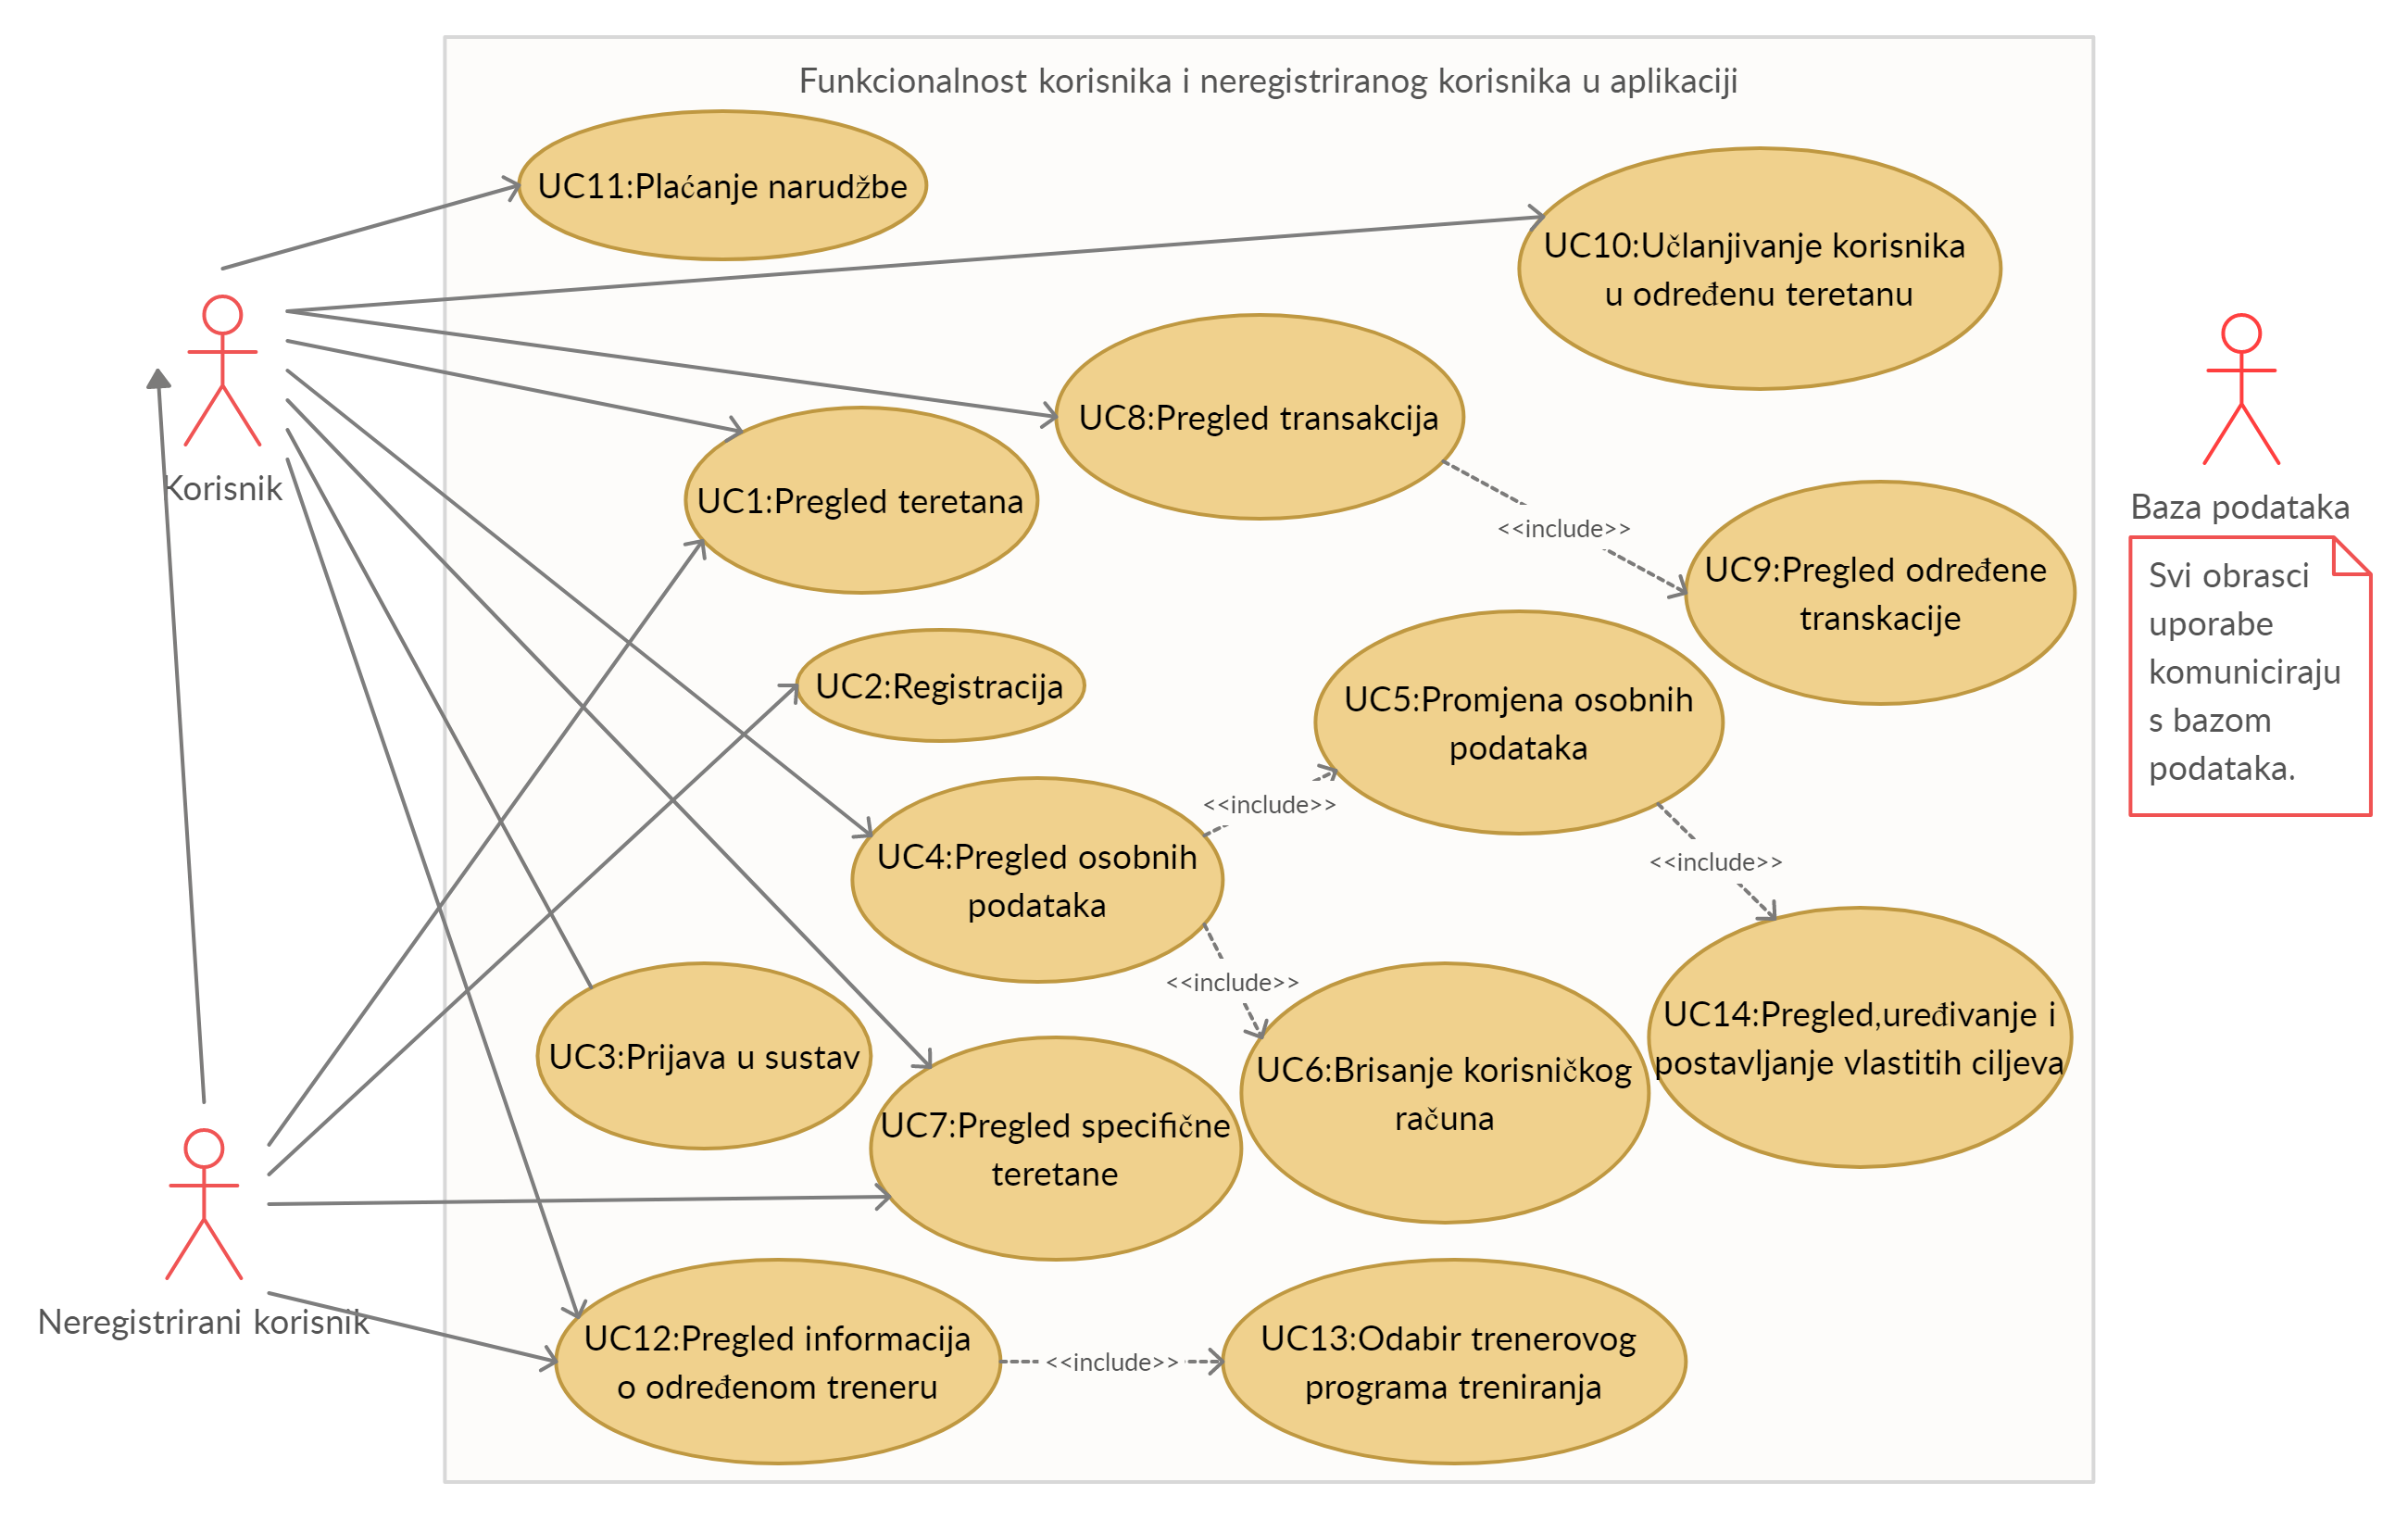
\includegraphics[height= 13cm,width=1.2\textwidth]{slike/obrazac1.jpg}
					\textbf{Slika 3.1: Dijagram obrasca uporabe, funkcionalnost korisnika i neregistriranog korisnika u aplikaciji  }
					
				\end{figure}
				
				\begin{figure}
					
					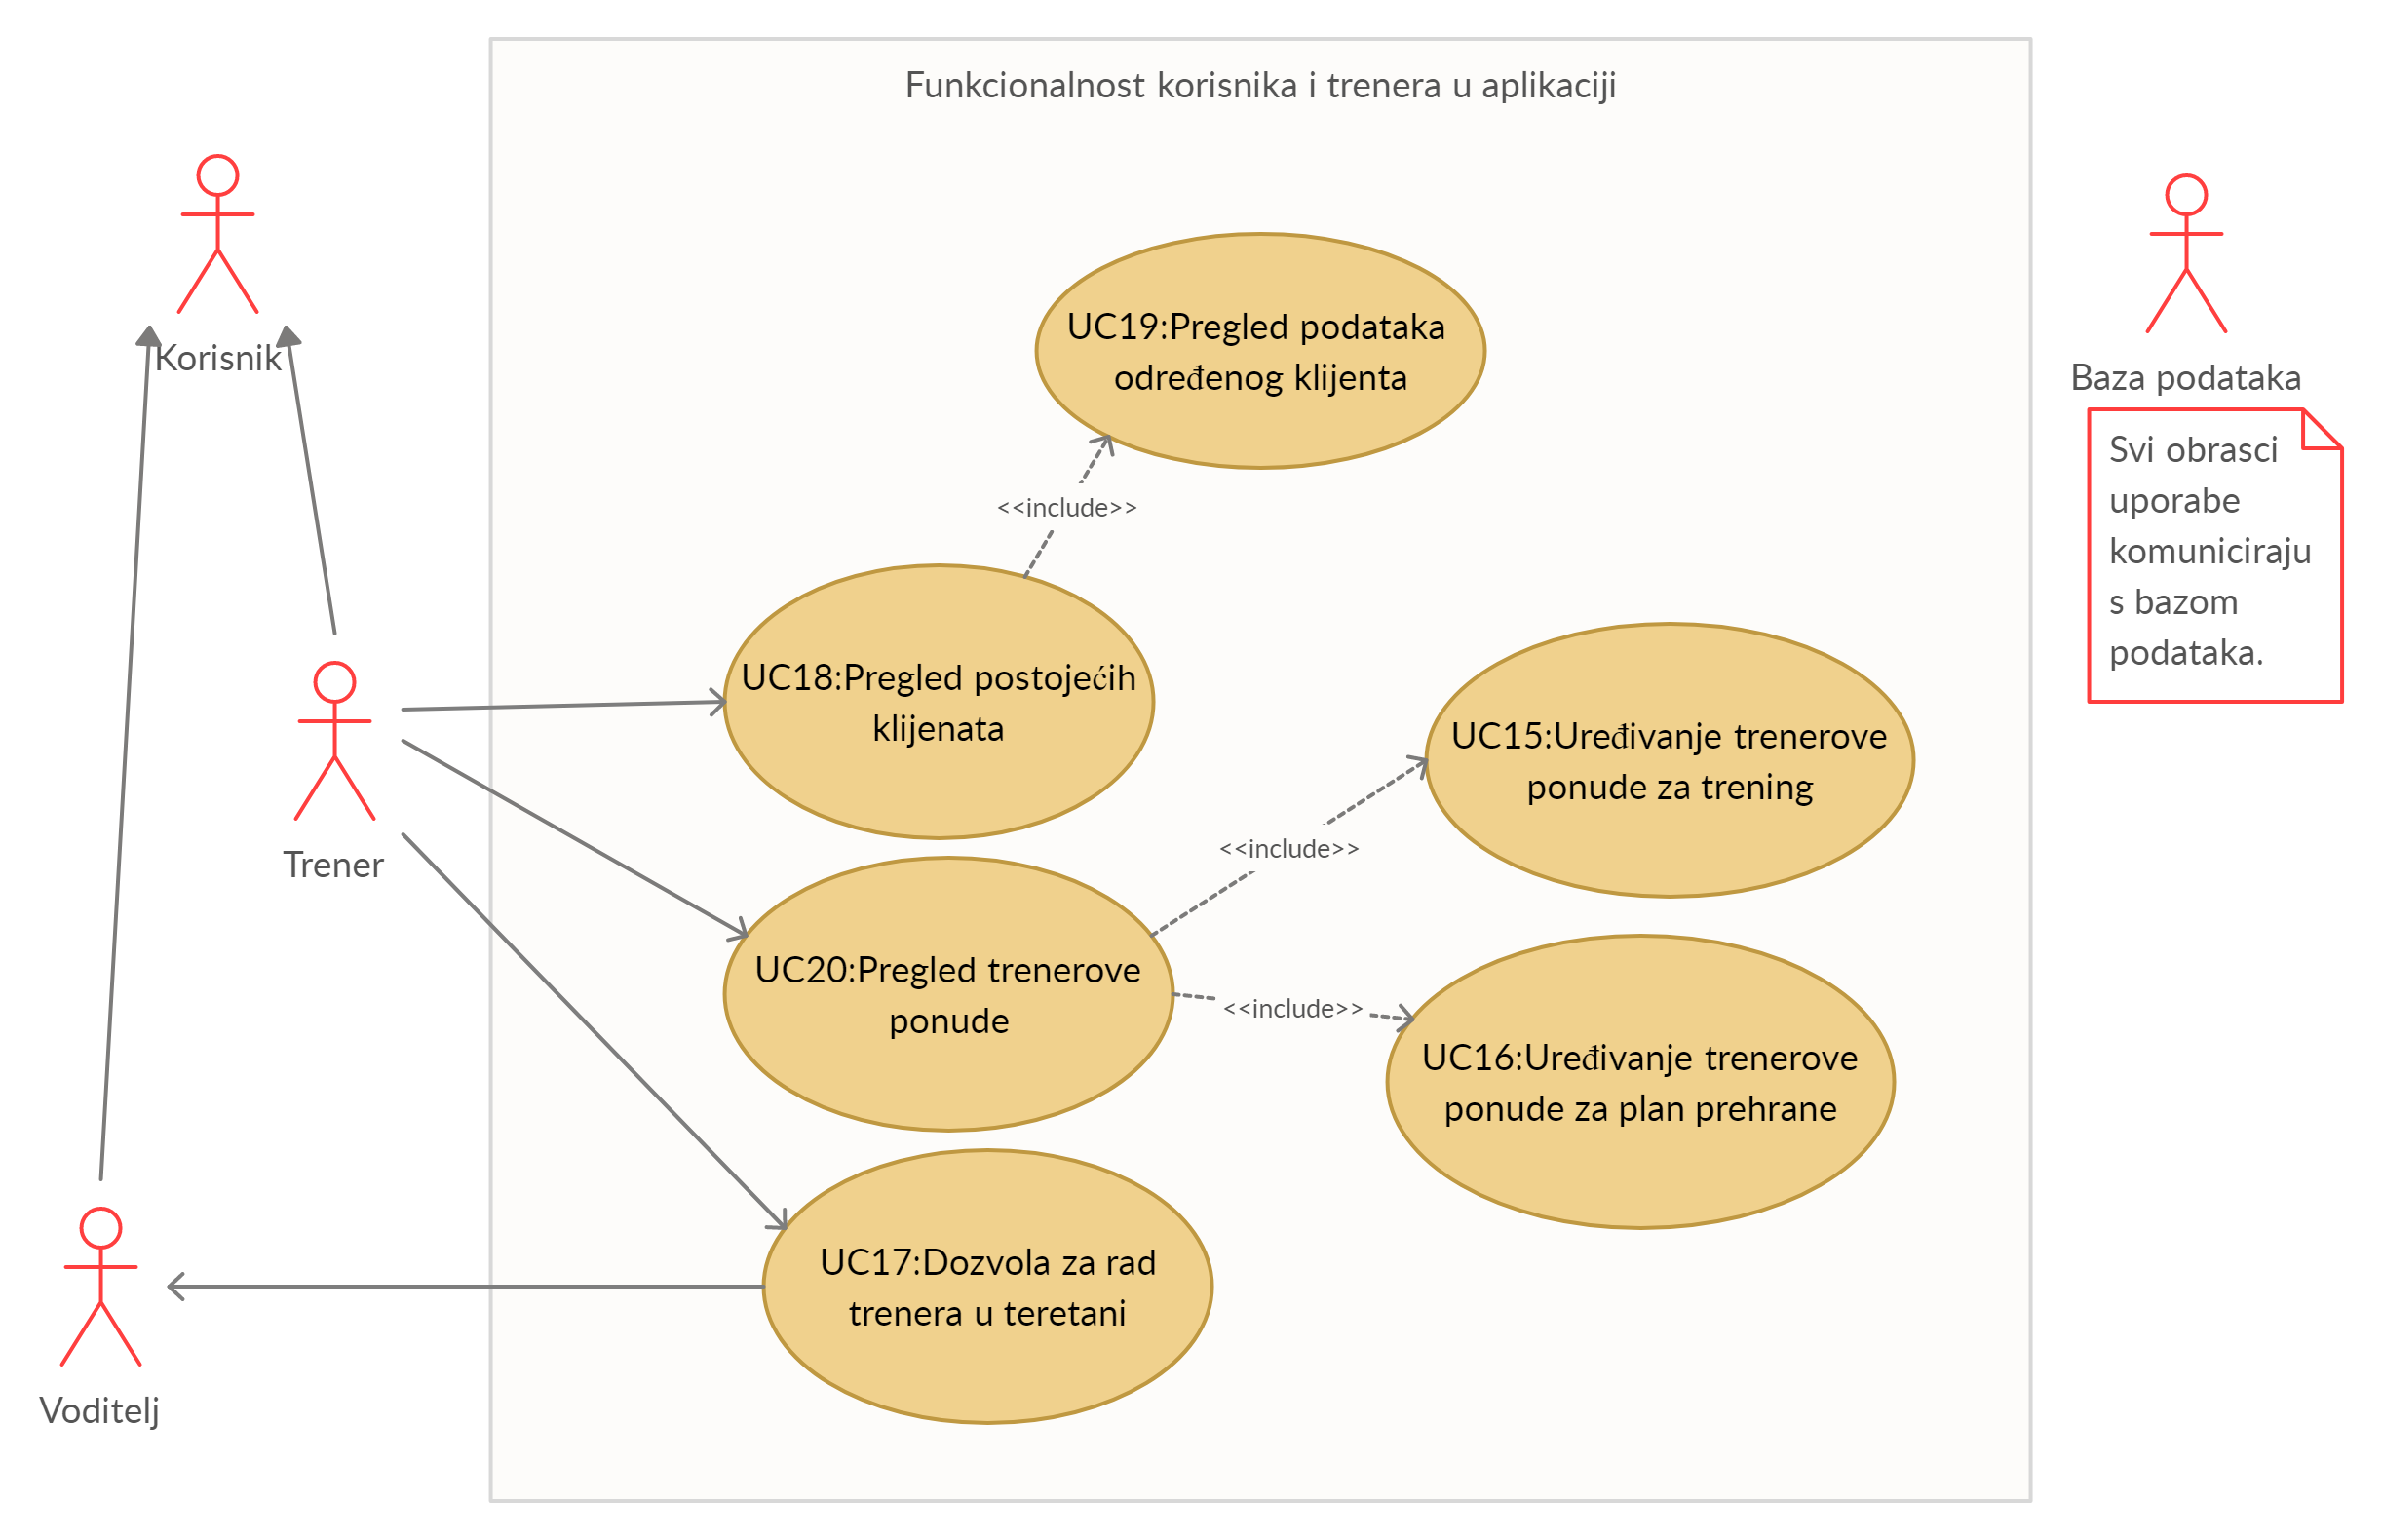
\includegraphics[height=13cm,width=1.2\textwidth]{slike/obrazac2.jpg}
					
					\textbf{Slika 3.2: Dijagram obrasca uporabe, funkcionalnost korisnika i trenera u aplikaciji}
				\end{figure}
				
				\begin{figure}
					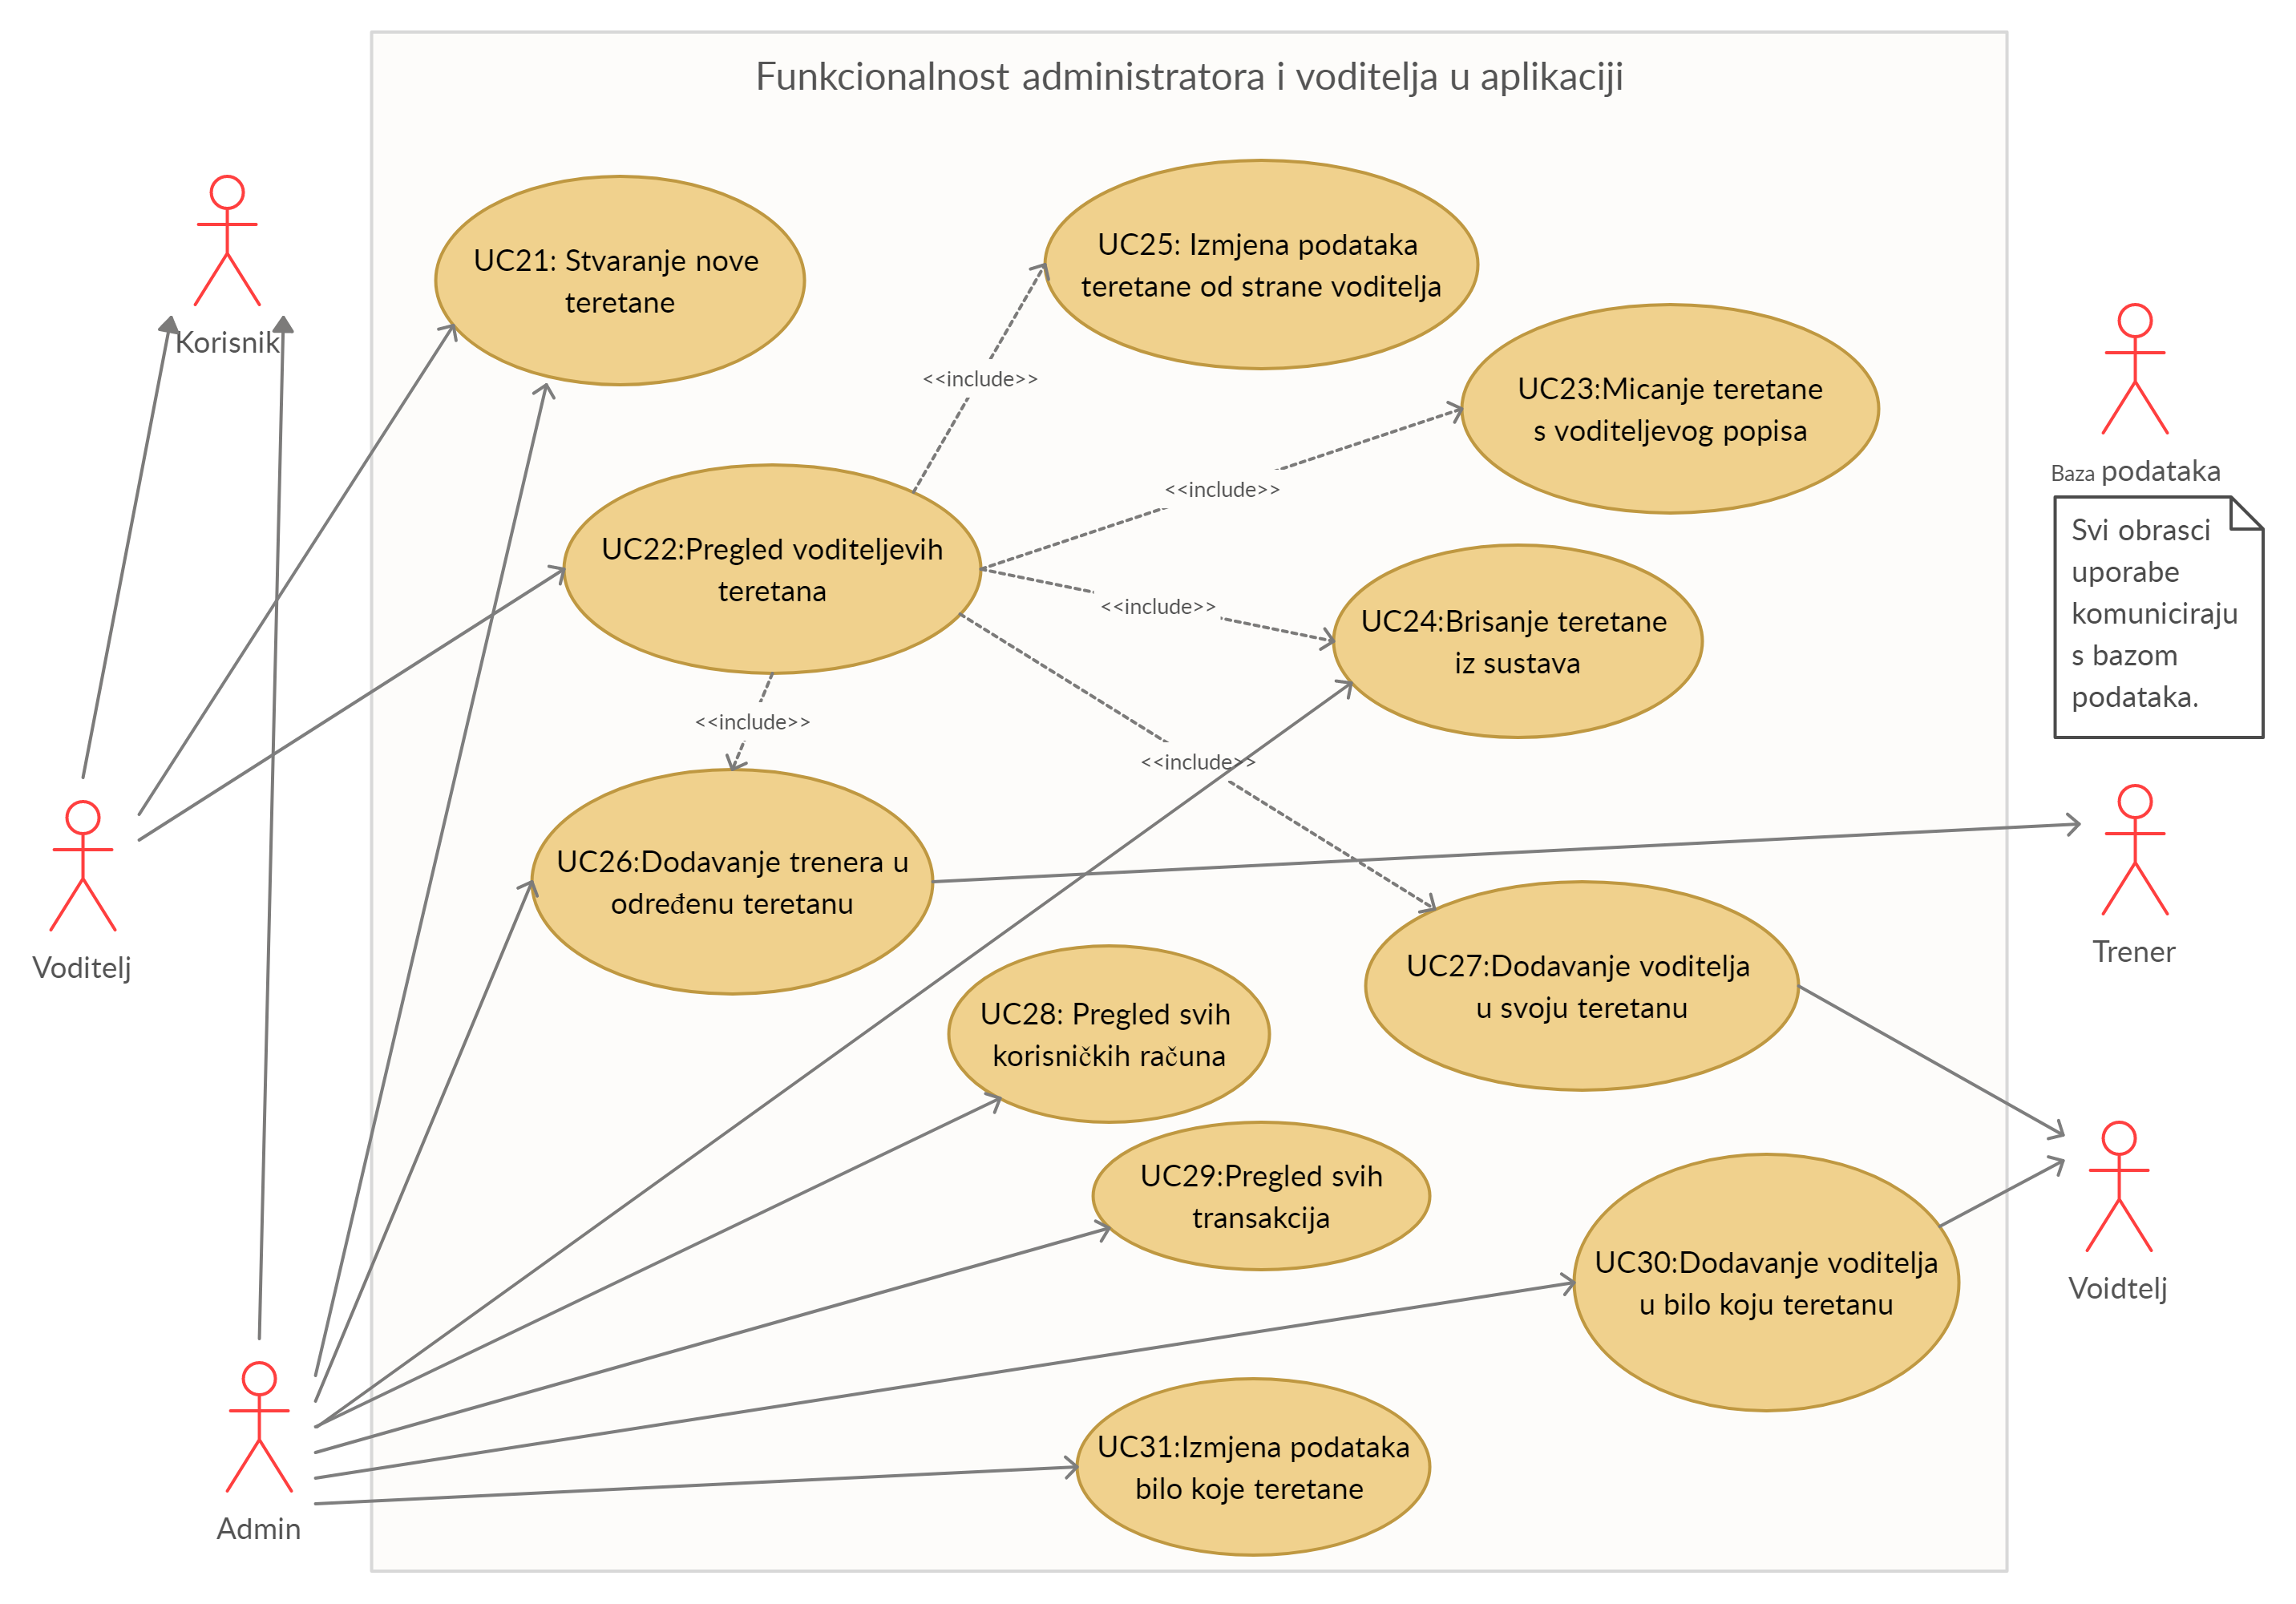
\includegraphics[height= 13cm,width=1.2\textwidth]{slike/obrazac3.jpg}
					\textbf{Slika 3.3: Dijagram obrasca uporabe, Funkcionalnost korisnika i neregistriranog korisnika u aplikaciji}
					
				\end{figure}
				
				
				\eject
					
				
			\subsection{Sekvencijski dijagrami}
				
				\textbf{\textit{dio 1. revizije}}\\
				
				\textit{Nacrtati sekvencijske dijagrame koji modeliraju najvažnije dijelove sustava (max. 4 dijagrama). Ukoliko postoji nedoumica oko odabira, razjasniti s asistentom. Uz svaki dijagram napisati detaljni opis dijagrama.}
				
					\subsubsection{Obrazac uporabe UC10 - Učlanjivanje korisnika u određenu teretanu (ili lanac teretana)}
					\textit{}Klijent šalje zahtjev za popis svih teretani te web aplikacija dohvaća popis teretana
                    iz baze podataka te prikazuje klijentu. Klijent potom odabire teretanu te mu se izlistava
                    popis članarina unutar odabrane teretane, tada klijent odabire članarinu koju želi te 
                    ako trenutno nema odabranu članarinu aktivnu dobiva poruku kako je članarina odabrana, 
                    dok ga u suprotnom Web aplikacija preusmjerava natrag na popis članarina za odabrati
                    iz odabrane teretane\\
                    
                    \begin{figure}[H]
			            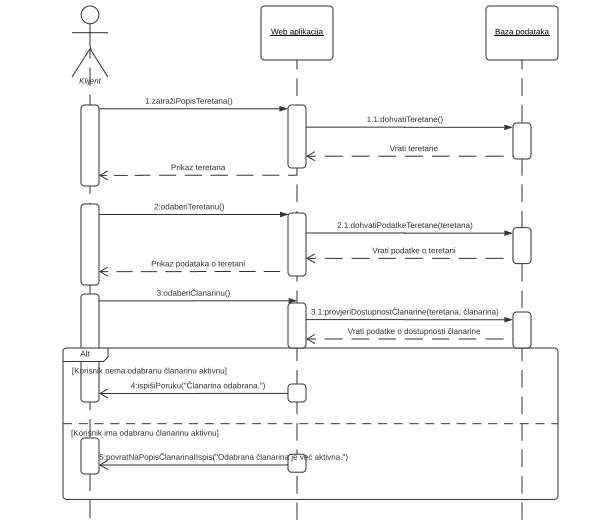
\includegraphics[scale=0.9]{slike/UC10.PNG} %veličina slike u odnosu na originalnu datoteku i pozicija slike
			            \centering
			            \caption{Sekvencijski dijagram za UC10}
			            \label{fig:promjene}
		            \end{figure}
                    
                    
                    \subsubsection{Obrazac uporabe UC13 - Odabir trenerovog programa treniranja ili plana prehrane}
					\textit{}Klijent šalje zahtjev za popis svih trenera te web aplikacija dohvaća popis trenera
                    iz baze podataka te ih sve prikazuje klijentu. Klijent potom odabire trenera. Tada
                    klijent ima opciju odabrati trening ili plan prehrane kod odabranog trenera. U slučaju
                    odabira plana prehrane plan prehrane se pokazuje korisniku. U slučaju odabira treninga,
                    korisnik uz trening odabire i termin treninga. Ako je termin slobodan korisnik dobiva tu
                    informaciju dok u suprotnom dobiva popis slobodnih termina treninga kod odabranog trenera
                    iz kojih potom bira novi termin.\\
                    
                    \begin{figure}[H]
			            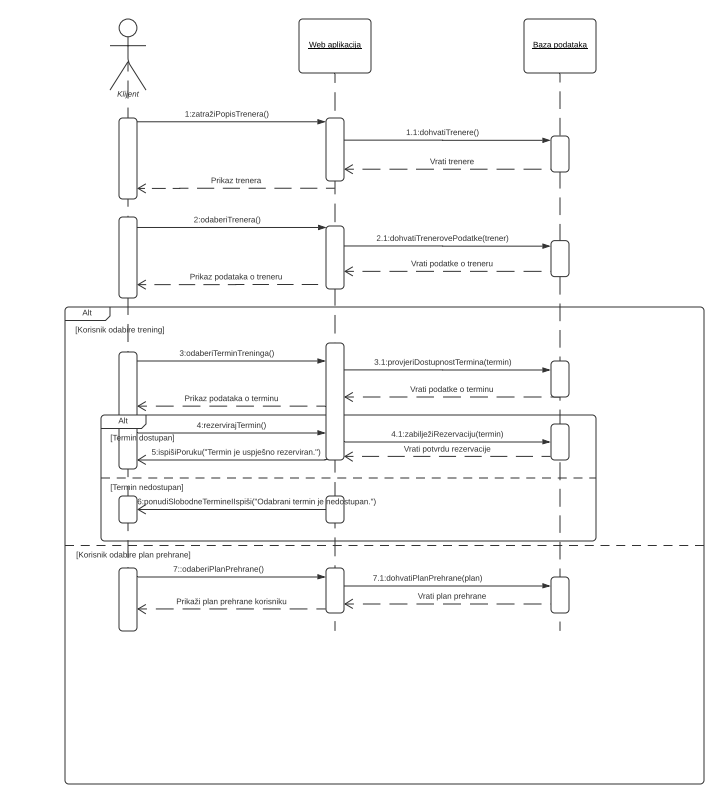
\includegraphics[scale=0.9]{slike/UC13.PNG} %veličina slike u odnosu na originalnu datoteku i pozicija slike
			            \centering
			            \caption{Sekvencijski dijagram za UC13}
			            \label{fig:promjene}
		            \end{figure}
                    
                    
                    \subsubsection{Obrazac uporabe UC15 - Uređivanje trenerove ponude za treninge}
					\textit{}Trener šalje zahtjev za popis svih njegovih programa te web aplikacija dohvaća popis
                    iz baze podataka te ih prikazuje treneru. Trener potom odabire jedan od ponuđenih programa
                    te web aplikacija iz baze podataka povlači informacije o programu te izlistava sve treneru.
                    Trener potom može izmjeniti program te se naknadno ta promjena zabilježava u bazu podataka
                    za buduće izmjene ili potražnje korisnika za tim programom.\\
                    
                    \begin{figure}[H]
			            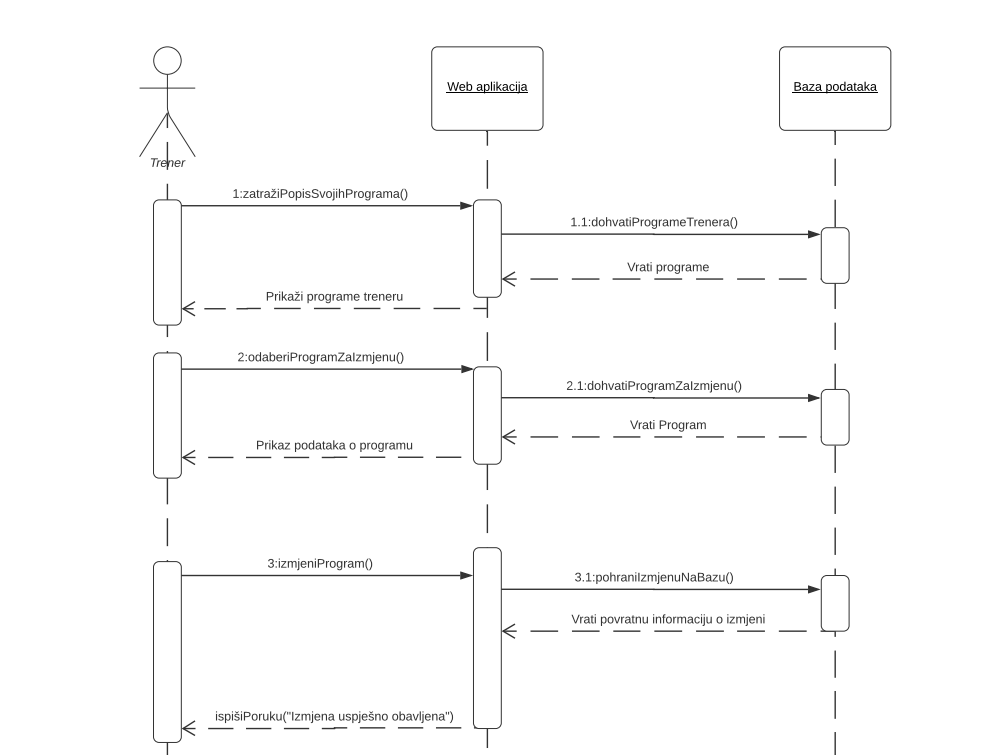
\includegraphics[scale=0.9]{slike/UC15.PNG} %veličina slike u odnosu na originalnu datoteku i pozicija slike
			            \centering
			            \caption{Sekvencijski dijagram za UC15}
			            \label{fig:promjene}
		            \end{figure}
                    
                    
                    \subsubsection{Obrazac uporabe UC17 - Dozvola za rad trenera u teretani}
					\textit{}Trener šalje zahtjev za popis svih teretani te web aplikacija dohvaća popis
                    iz baze podataka te ih prikazuje treneru. Trener potom odabire teretanu za 
                    koju je zainteresiran, a podaci o teretani se ponovo dohvaćaju iz baze podataka.
                    Tada trener šalje zahtjev za rad u teretanu, a web aplikacija u bazi provjerava
                    radi li već trener u odabranoj teretani. U slučaju da ne radi u odabranoj teretani
                    dobiva poruku kako je zahtjev uspješno zaprimljen te zahtjev čeka odobrenje voditelja
                    teretane, a u slučaju da trener ondje već radi dobiva poruku koja ga o tome obavještava.\\
                    
                    \begin{figure}[H]
			            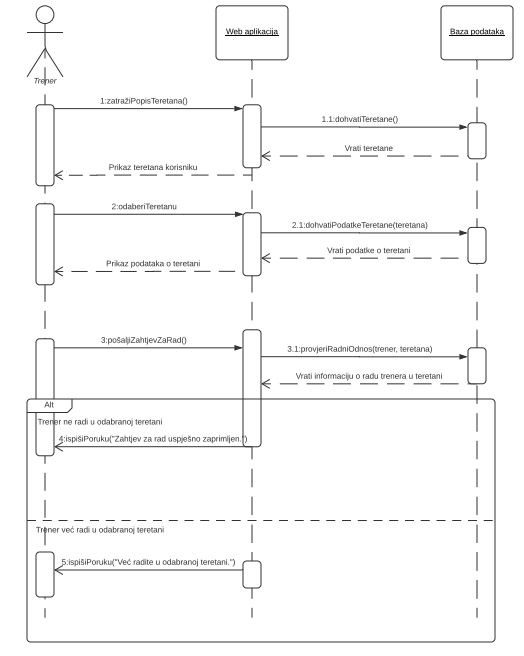
\includegraphics[scale=0.9]{slike/UC17.PNG} %veličina slike u odnosu na originalnu datoteku i pozicija slike
			            \centering
			            \caption{Sekvencijski dijagram za UC17}
			            \label{fig:promjene}
		            \end{figure}
                    
				
				
				\eject
	            
	            
	            
		\section{Ostali zahtjevi}
		
			\begin{itemize}
	        	\item 	Sustav treba podržati rad više korisnika u stvarnom vremenu bez gubitaka funkcionalnosti
	        	\item 	Prikaz i tekstualni unos mora podržavati hrvatske dijakritičke znakove
	        	\item 	Sustav treba biti jednostavan za korištenje, korisnici se moraju znati koristiti web sučeljem i sustavom bez opširnih uputa 
	        	\item 	Sustav bi trebao jamčiti točnost i pouzdanost informacija u aplikaciji
	        	\item 	Ažuriranje i nadogradnja sustava ne smije narušavati postojeće funkcionalnosti sustava
	        	\item 	Baza podataka mora biti brza i zaštićena od bilo kakvih vanjskih utjecaja
	        	\item 	Odgovor na korisnikov upit koji je povezan sa bazom podatak bi trebao biti najduže par sekundi
	        	\item 	Nepravilne akcije korisnika, trenera ili voditelja u korisničkom sučelju ne smiju narušiti postojeće funkcionalnosti sustava
	        	\item 	Sustav kao valutu dopušta hrvatsku kunu
	        	\item 	Sustavu se treba moći pristupiti iz javne mreže sigurnim protokolom(HTTPS)
        	\end{itemize}
